In this chapter, we present the experimental results of our performance and energy-efficiency evaluation of modern datacenter AI accelerators. Following the structure introduced in Chapter~\ref{chap:methods}, we organise the discussion into three parts: Single-GPU experiments (Section~\ref{chap:results:sec:single}), Multi-GPU experiments (Section~\ref{chap:results:sec:multi}), and an analysis of dataflow AI accelerators (Section~\ref{chap:results:sec:dsa}).


\section{Single GPU Experiments}
\label{chap:results:sec:single}

In this section, we discuss the performance of LLM inference on a single GPU, comparing six different GPUs from Nvidia, AMD, and Intel.
We analyze three key performance metrics: End-to-end latency, Time to First Token (TTFT), and Throughput.
For energy efficiency, we utilize Tokens per Joule as the metric.

\ref{fig:all_metrics_1gpu} shows how performance and energy efficiency evolve with batch size across 6 different GPUs and four LLM models running with half (16-bit) precision. Multi-Tile GPUs (AMD MI250 and Intel Max 1550) use tensor parallelism to fully utilize their resources.
From those experiments, we can extract three main insights: 
(1) a cross-vendor comparison of the performance and energy efficiency of GPU models, \
(2) the trend of performance and energy efficiency as model size grows, and 
(3) the trade-off between latency and throughput across different batch sizes.

\begin{figure}[h]
    \centering
    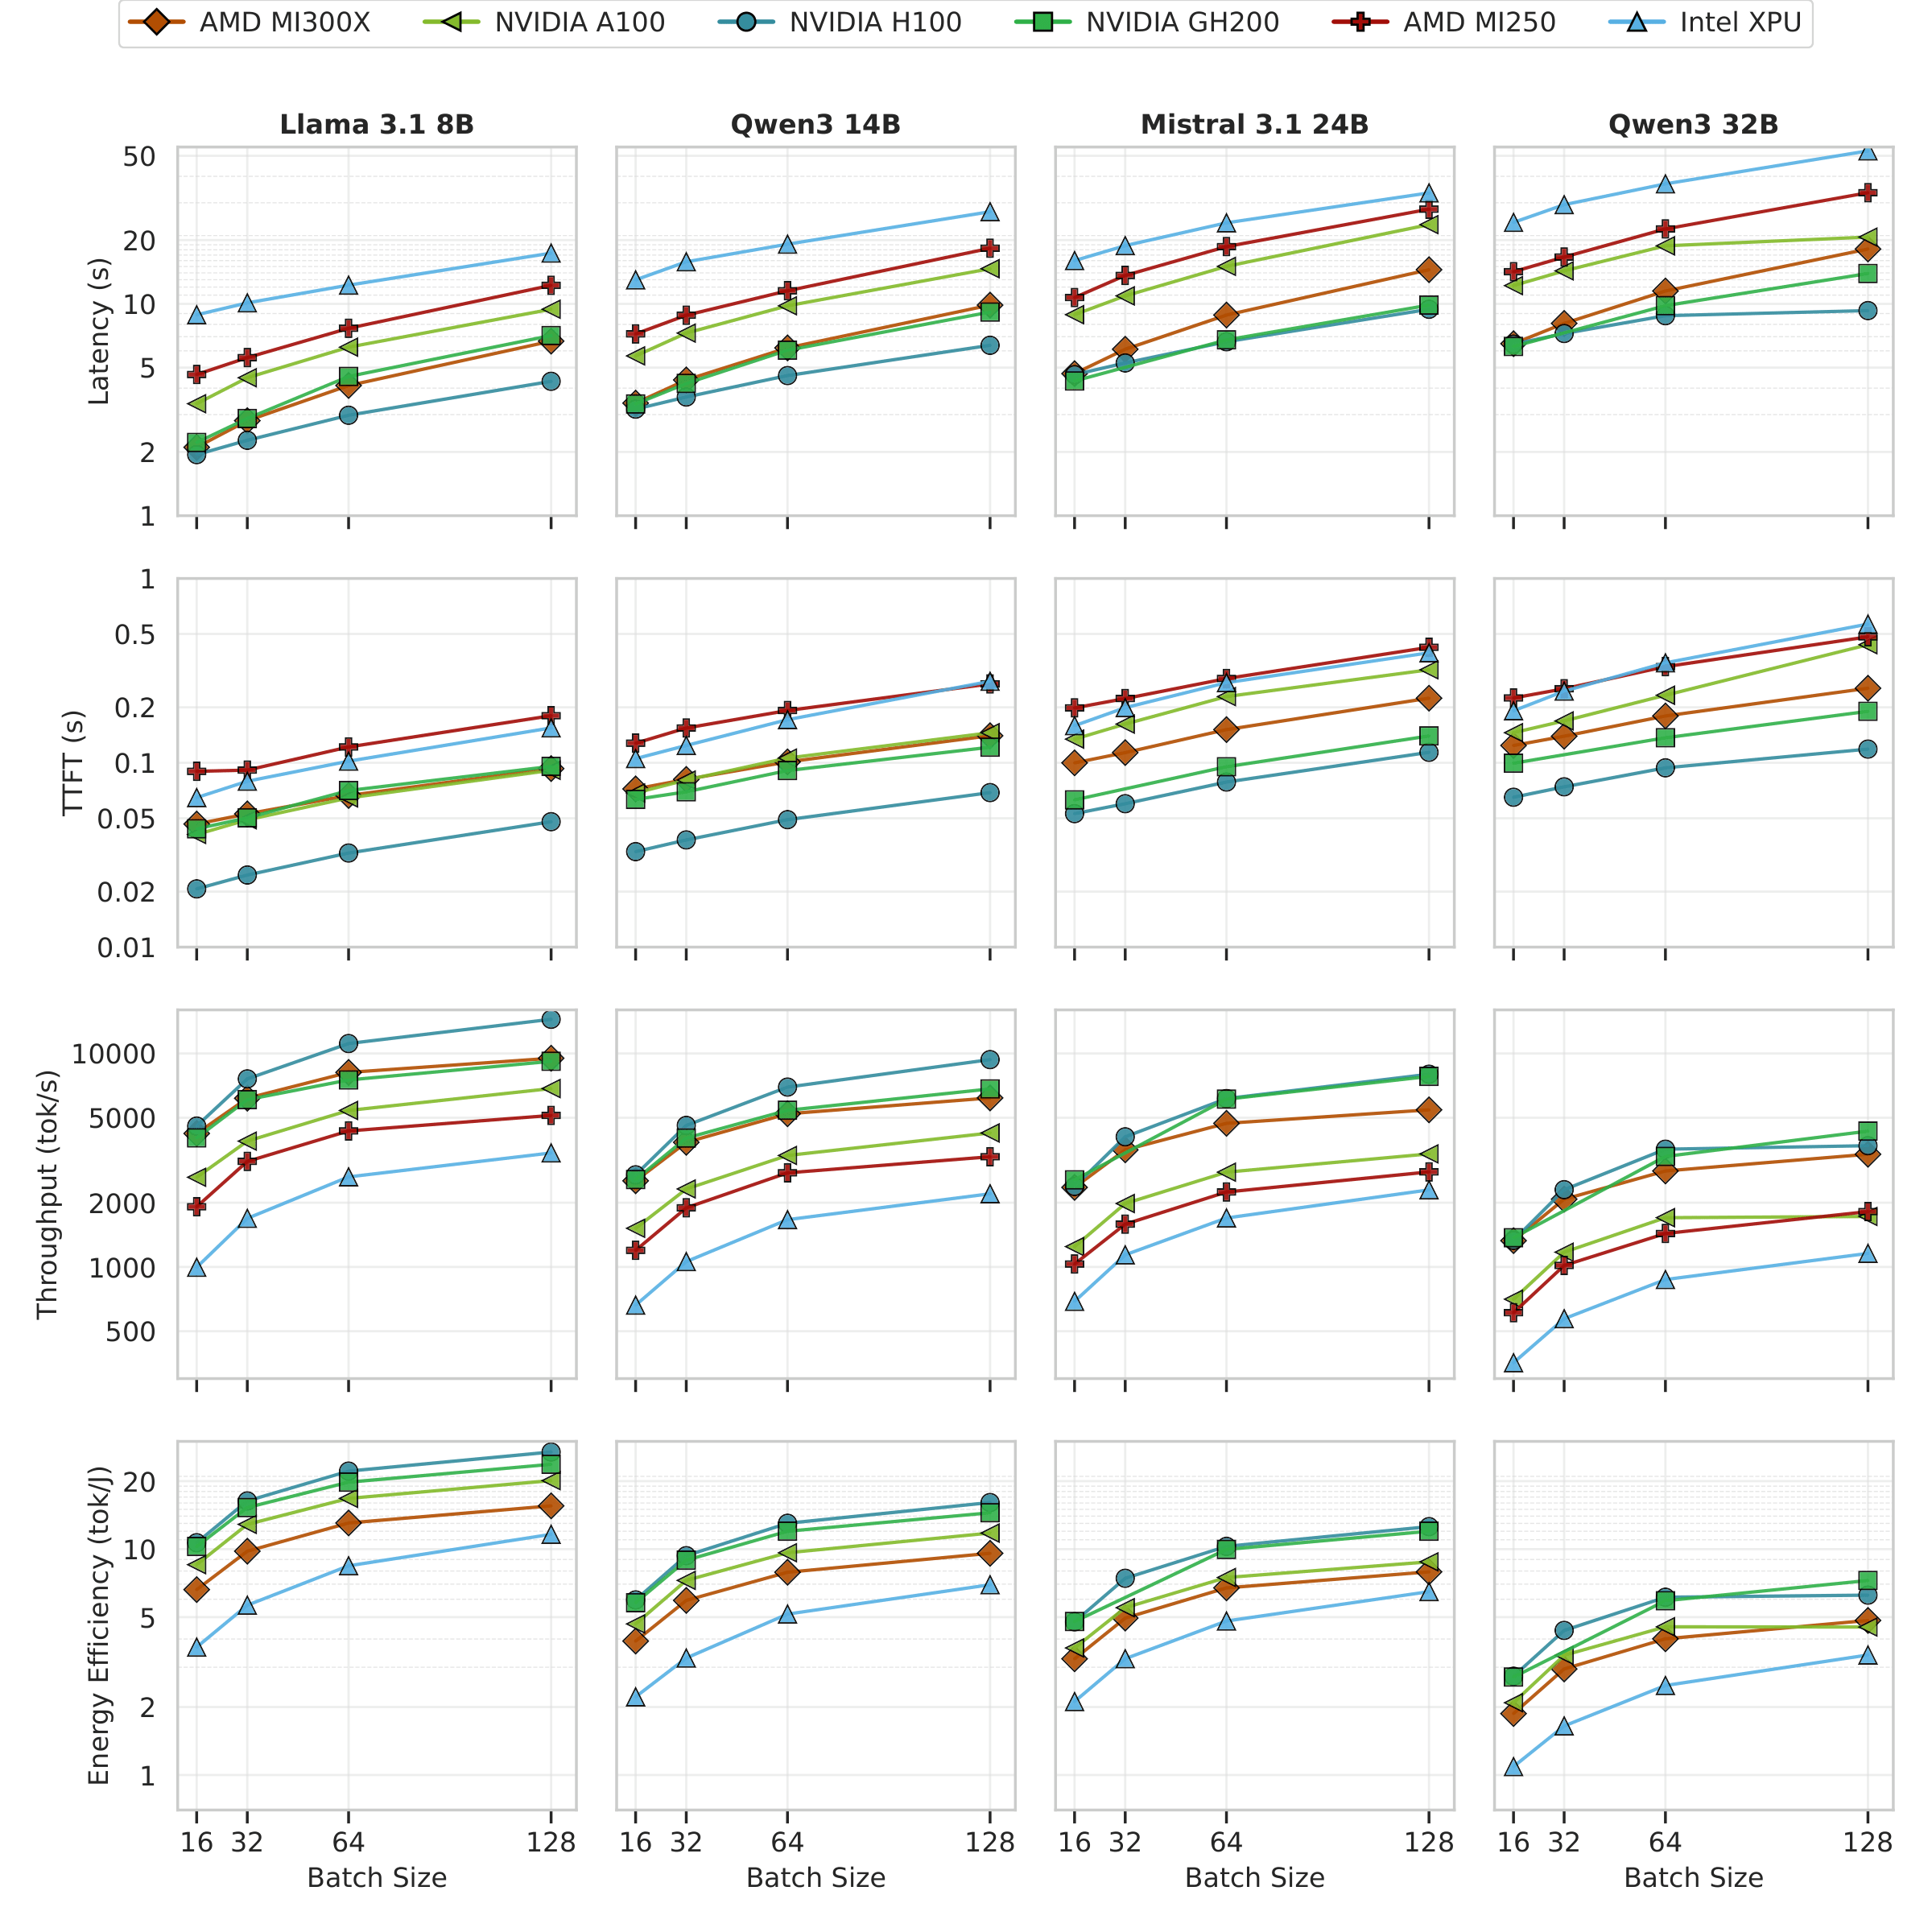
\includegraphics[width=\textwidth]{figs/combined_performance_plots.png}
    \caption{The evolution of performance and energy efficiency with batch size across six GPUs.}
    \tagpdfsetup{alttext={The evolution of performance and energy efficiency with batch size across six GPUs.}}
    \label{fig:all_metrics_1gpu}
\end{figure}

\subsection{GPU model comparison}
For this analysis, we use the NVIDIA A100 as the natural performance baseline, as it is both the oldest and most widely used GPU among those tested. Both Nvidia Hopper (H100 and GH200) and AMD CDNA3 (MI300x) GPUs consistently outperform the A100 baseline in terms of performance, across models and batch sizes. The AMD MI250 and the Intel Max 1550, instead, are both outperformed by the Ampere GPU. Importantly, both GPUs feature larger memories than their Nvidia counterparts (128 GB compared to 80 GB), which leads to two main benefits. First, they support running larger models, and second, they substantially narrow the throughput gap as model size and batch size increase. In fact, especially with the larger 32B model, Nvidia A100 and H100 saturate their throughput at batch size 64 due to the insufficient memory available for KV cache.
Concerning the increased latency and the lower throughput, it is also important to mention that each Intel Max 1550 and AMD MI250 is constituted of two GPU tiles and thus requires frequent all-gather operations between the two to fully utilize its compute power. This is particularly detrimental in small models, advantaging monolithic GPUs.

Regarding energy efficiency, Nvidia Hopper GPUs demonstrate an improvement over the previous generation, despite their increased average power consumption. In fact, where the Nvidia A100 had a TDP of 400W and an average power consumption of 337W, the Nvidia H100 has a TDP of 700W and consumes, on average, 478W. Nevertheless, the substantial decrease in latency is sufficient to compensate for the increased power consumption.
The same does not hold for AMD MI300x, which consistently surpasses the A100 in raw performance but achieves lower energy efficiency. Notably, the AMD MI300x has the highest power consumption among the GPUs tested (750W TDP and 625W average power consumption).
The Intel Max 1550 exhibits higher latency and increased power consumption compared to the Nvidia A100, resulting in lower energy efficiency.

AMD MI250 and Intel Max 1550 underperform relative to the NVIDIA A100 despite their higher power consumption. This gap is partly due to their multi-tile designs, which require tensor parallelism to fully utilize the hardware, as each tile is presented to the operating system as a separate device. Additionally, the AMD and Intel implementations of vLLM currently lag in software maturity, lacking support for key optimizations. In terms of energy efficiency, the Intel Max 1550 is less efficient than the A100, while no data is available for the AMD MI250.

Memory capacity is another critical factor. NVIDIA GPUs rank lowest in VRAM, which limits the size of models they can host compared to the other GPUs under analysis. The AMD MI300x provides the largest memory capacity at 192GB, enabling a single device to run 70B-parameter models. It is also important to note that the current vLLM implementation does not utilize all the unified memory of the GH200 SoC, which limits the memory capacity to 96 GB of VRAM, resulting in comparable performance to the base NVIDIA H100.

NVIDIA Hopper GPUs emerge as the most performant and energy-efficient GPU among those tested. The AMD MI300X also displays competitive performance, outpacing the NVIDIA A100 in terms of performance, but not in energy efficiency. Intel Max 1550 and AMD MI250 offer lower performance and energy efficiency than NVIDIA A100.

\begin{figure}[H]
    \centering
    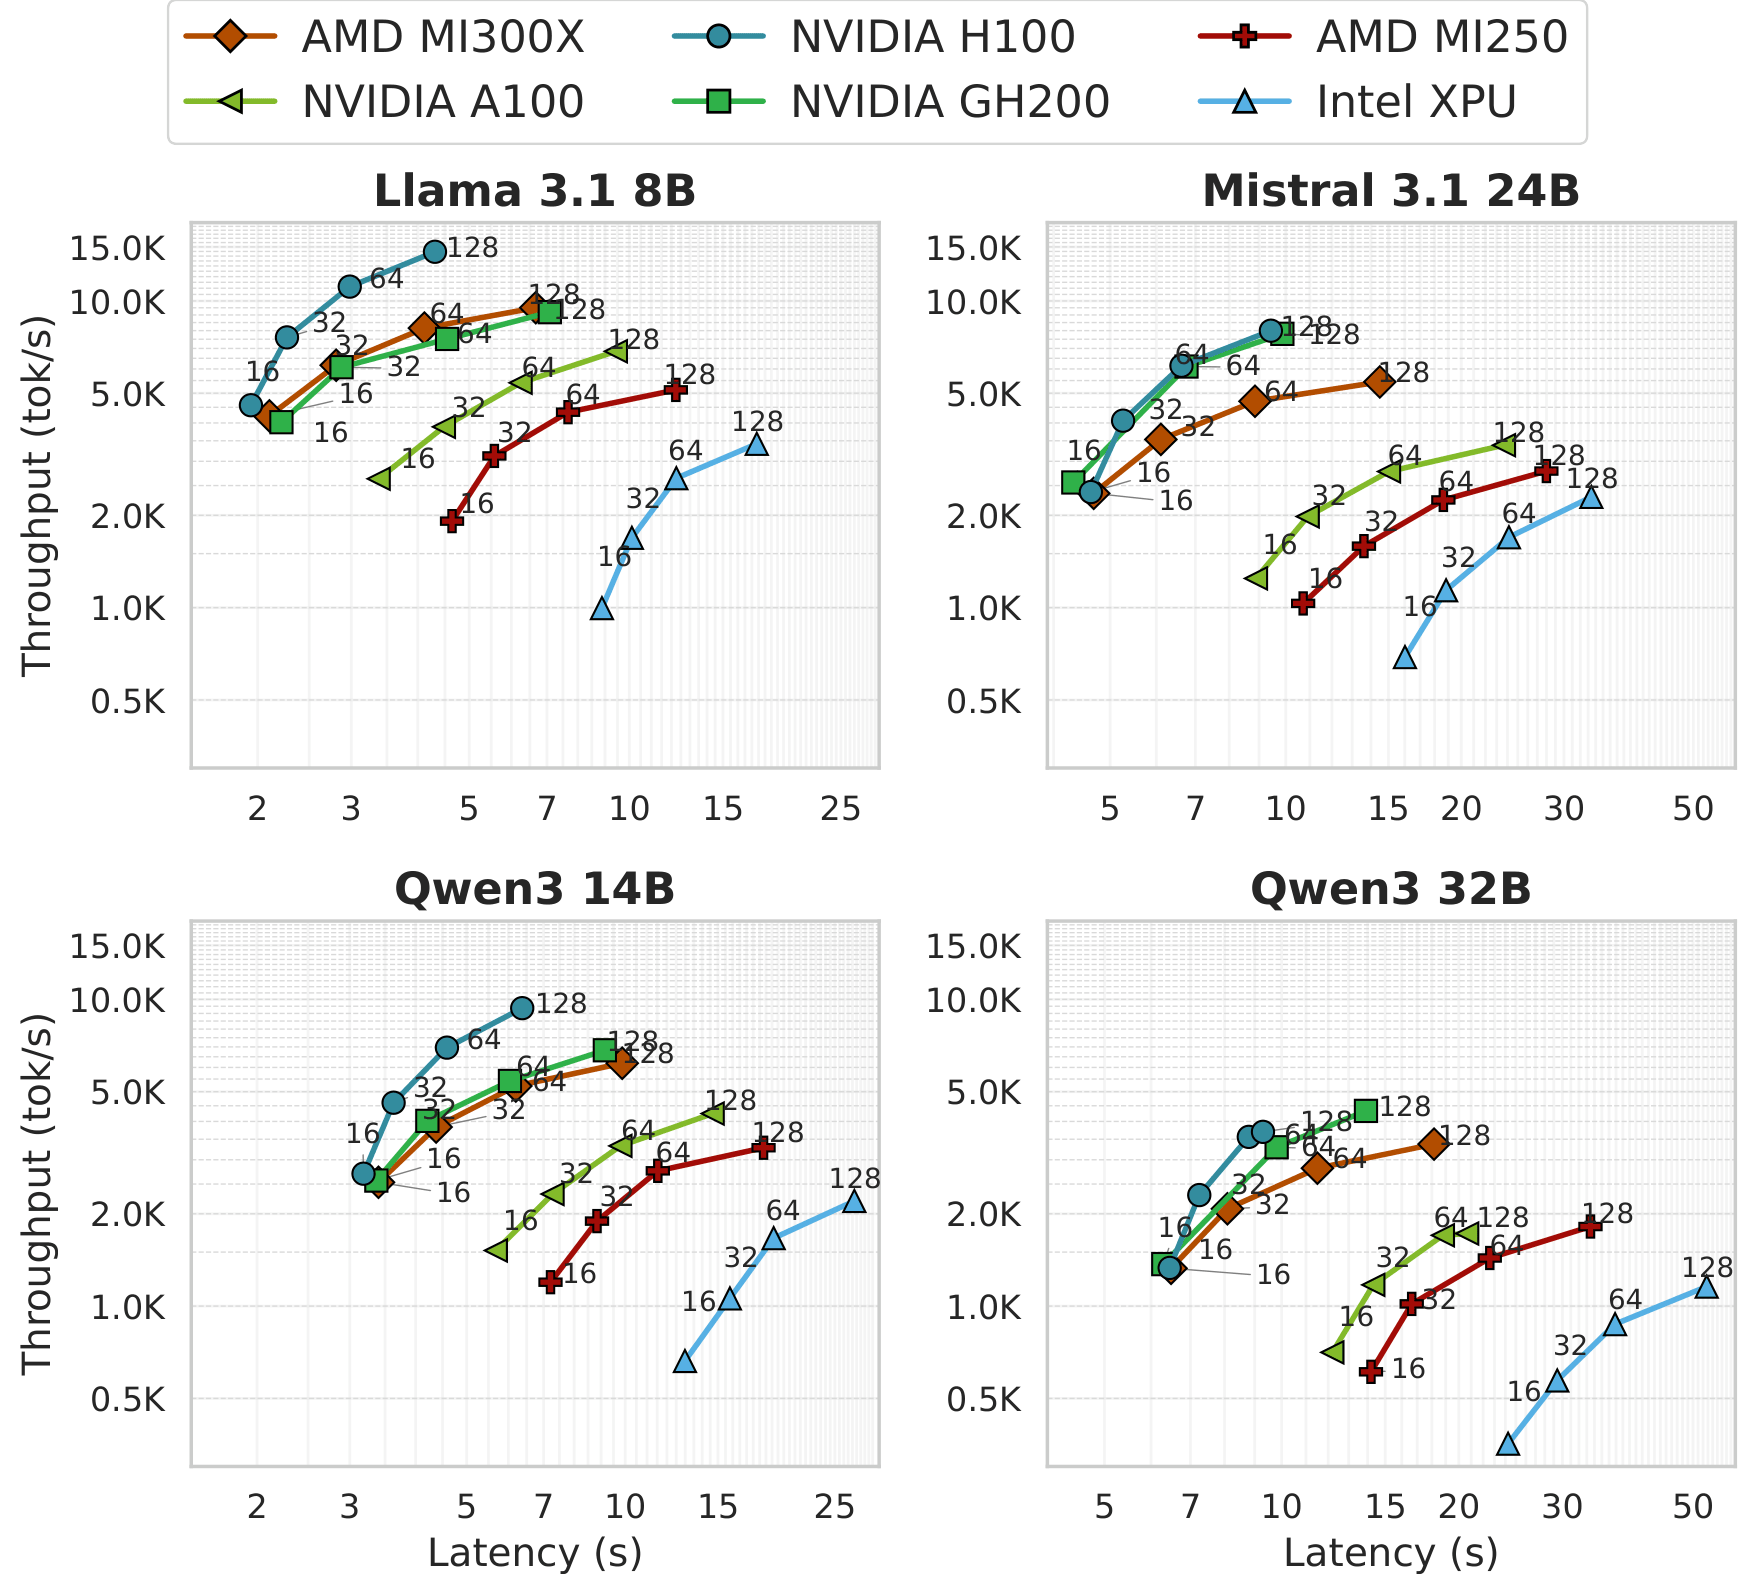
\includegraphics[width=0.9\textwidth]{figs/throughput_latency_plot.png}
        \caption{Trade-off between throughput and latency across batch sizes (16-128), using four LLM models and six different GPUs. The numbers in the plots indicate the batch sizes.}
        \tagpdfsetup{alttext={Trade-off between throughput and latency across batch sizes (16-128), using four LLM models and six different GPUs. The numbers in the plots indicate the batch sizes.}}
    \label{fig:bs}
\end{figure}

\subsection{Batch Size} 
\ref{fig:bs} presents a different perspective on our evaluation data, enabling us to better understand the impact of batch size. The x-axis represents the average end-to-end latency of sequences, while the y-axis represents throughput. These representations allow us to observe the trade-off that happens under varying batch sizes.
Consistent with the analysis in Chapter \ref{chap:methods:sec:model}, we observe that across all GPU models, smaller batches result in lower latency due to reduced computation at each forward pass.
In fact, the number of FLOPs to be executed at each forward pass scales linearly with batch size $b$. However, the model weights have to be loaded from off-chip memory independently of $b$. This causes the compute-related part of latency to decrease linearly with batch size, while the operational intensity $OI$ (expressed in FLOPs/byte) drops linearly with $b$, making computation more memory-bound and thus harming throughput.

Increasing throughput also strongly correlates with improving energy efficiency.
After adjusting the GPU model and precision, we observe a correlation of 0.92 to 0.99 between energy efficiency and throughput. This is because batch size has a reduced impact on power consumption, whereas it has a significant effect on latency.

From these observations, we conclude that larger batch sizes improve the performance in an offline setting while also achieving better energy efficiency.
In contrast, metrics related to online serving, such as TTFT, ITL, or E2E latency, improve as the batch size decreases, creating a trade-off with energy efficiency. 

\begin{figure}[H]
    \centering
    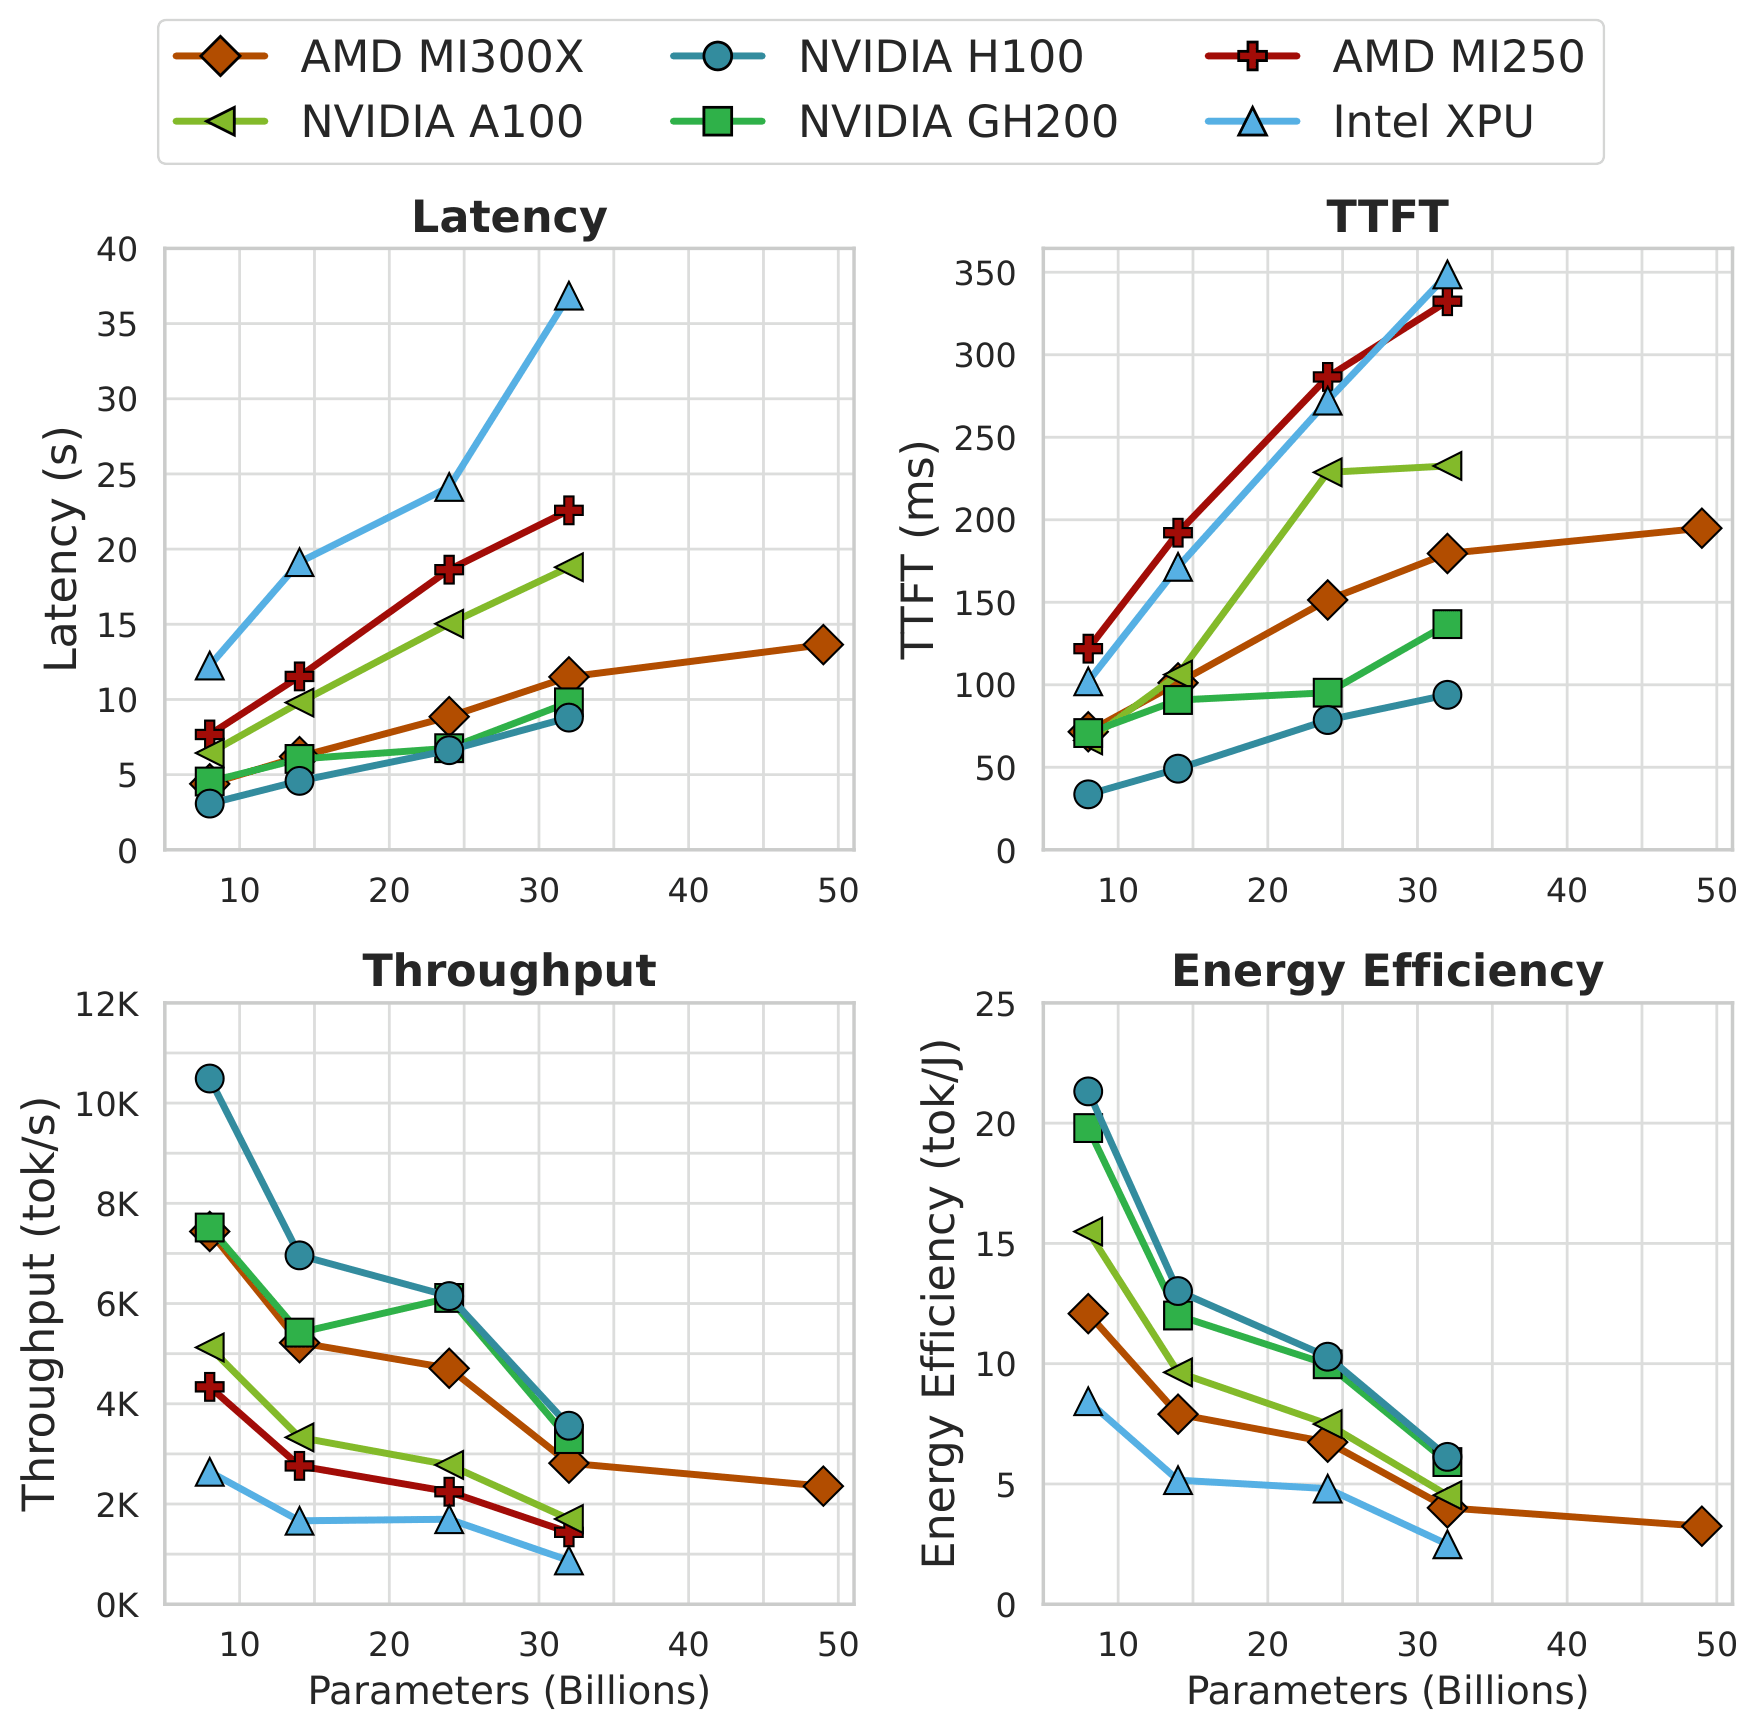
\includegraphics[width=0.7\textwidth]{figs/trend_Latency_TTFT_Throughput_Energy.png}
    \caption{Performance and energy efficiency across six GPUs for models of varying size.}
    \tagpdfsetup{alttext={Performance and energy efficiency across six GPUs for models of varying size.}}
    \label{fig:1gpu_modelsize}
\end{figure}

\subsection{Model Size} 
\ref{fig:1gpu_modelsize} displays a subset of the datapoints from \ref{fig:all_metrics_1gpu}, allowing us to better visualize how the four key metrics analyzed change as the model size increases, with the input dataset and batch size set to 64. 

As a first observation, we can see that latency and TTFT increase linearly with model size, while throughput and energy efficiency decrease inversely.
This trend is consistent with the analysis made in Chapter \ref{chap:methods:sec:model}, which predicts the latency of the forward pass to scale roughly linearly with the model size $N$.

\begin{comment}
\begin{figure}[H]
    \centering
    \includegraphics[width=0.9\textwidth]{figs/fp8_vs_bf16_improvements_subplots.png}
        \caption{  Throughput and energy-efficiency gains (FP8 vs. bfloat16) across four LLM models and four GPUs. The greatest improvement is annotated.}
    \label{fig:fp8}
\end{figure}
\end{comment}

\begin{figure}[H]
    \centering
    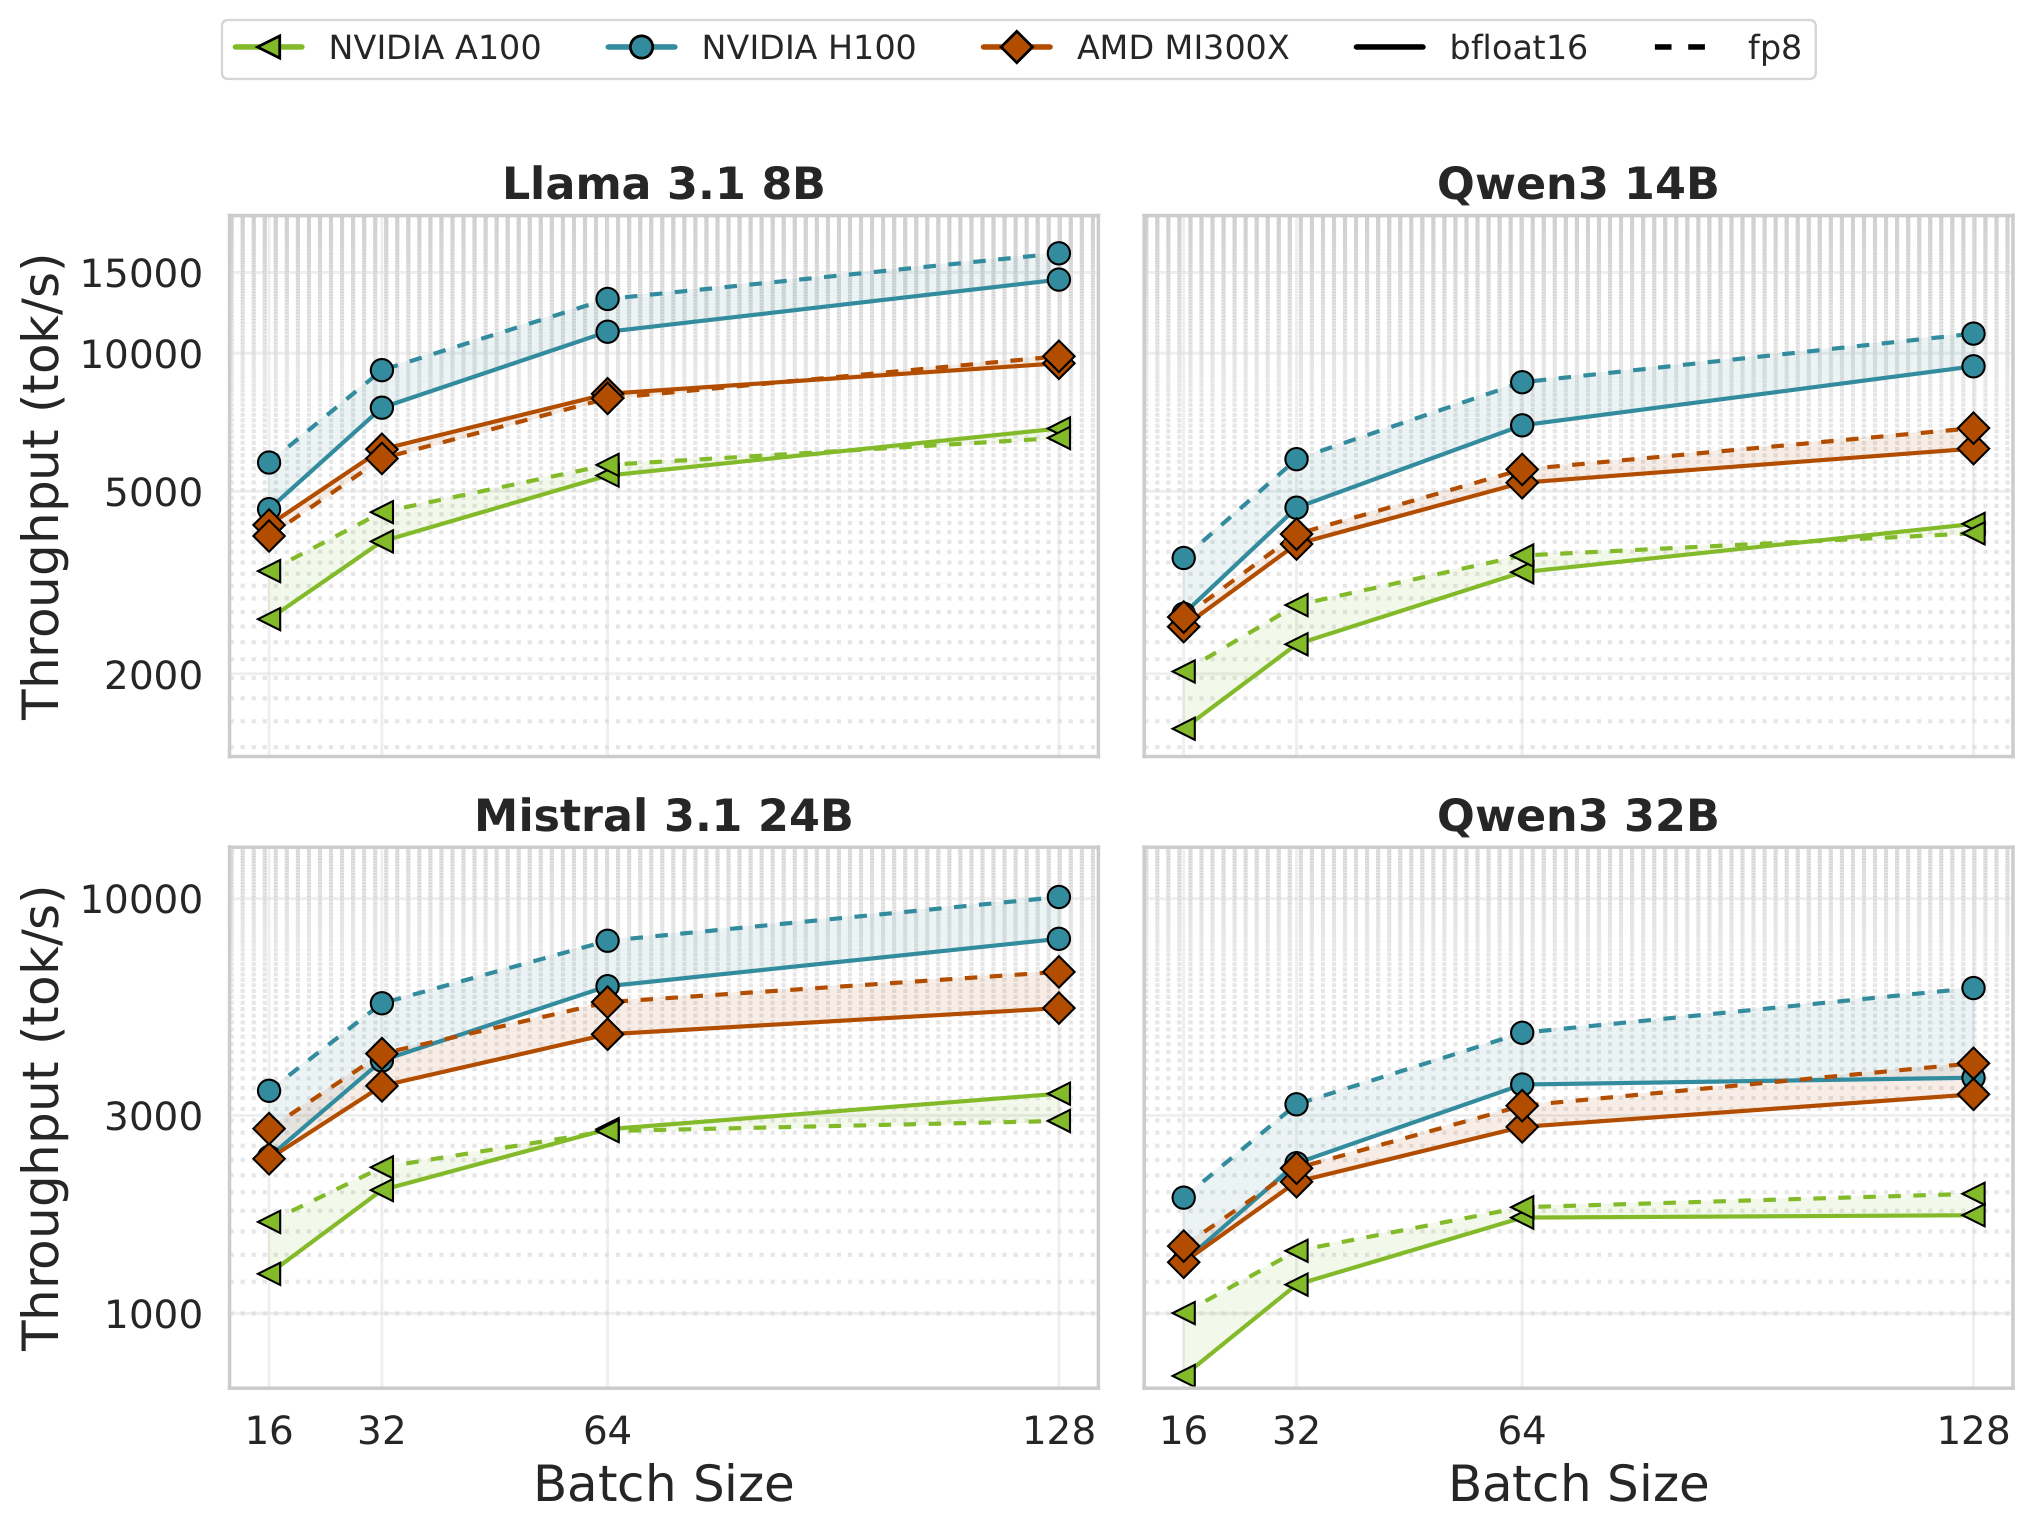
\includegraphics[width=\textwidth]{figs/throughput_by_model_with_precisions_filled.png}
    \caption{Throughput (tok/s) comaprison between bfloat16 and FP8 precision across GPUs and LLM models.}
    \tagpdfsetup{alttext={Throughput (tok/s) comaprison between bfloat16 and FP8 precision across GPUs and LLM models.}}
    \label{fig:fp8bs}
\end{figure}

\subsection{FP8 Quantization}

We evaluate the impact of FP8 quantization on throughput and energy efficiency across four GPU architectures: NVIDIA A100, H100, GH200, and AMD MI300X. \ref{fig:fp8bs} summarizes the results.

NVIDIA A100 does not provide native FP8 support and therefore relies on W8A16 quantization, which applies 8-bit weights and 16-bit activations. Although it cannot exploit FP8-specific functional units, A100 still benefits from the reduced memory footprint of 8-bit weights. In contrast, NVIDIA Hopper (H100, GH200) and AMD MI300X implement FP8 arithmetic natively and can operate with W8A8 precision throughout, yielding more substantial performance gains.

In theory, reducing precision from bfloat16 to W8A8 halves both the arithmetic cost and data movement, suggesting a near 2 $\times$ speedup. In practice, our measurements show that real-world improvements fall well short of this idealized limit. While W8A8 consistently outperforms bfloat16, the magnitude of gains varies significantly across hardware.

NVIDIA Hopper GPUs benefit the most, with throughput improvements of 20\%–38\% and energy-efficiency gains of 34\%–46\%. AMD MI300X shows smaller and more model-dependent improvements: throughput ranges from no gain on Llama 8B to roughly 20\% on Mistral Small 24B; energy efficiency improves by 16\%–35\%. These results highlight the gap between theoretical and practical benefits, underscoring the need for hardware–software co-design to fully exploit low-precision arithmetic.

Batch size also plays an important role. W8A8 quantization becomes increasingly advantageous at larger batch sizes, where arithmetic dominates execution time. Conversely, W8A16 (used on A100) yields its largest gains at small batch sizes, where the workload is more memory-bound, and exhibits diminishing returns as the batch size increases. \ref{fig:fp8bs} illustrates these trends for Qwen3 32B.

Quantization inevitably introduces some loss in model accuracy. While a complete analysis is left for future work, prior results \cite{kurtic2024give} indicate that FP8-quantized models retain more than 99\% of the accuracy of their bfloat16 counterparts on standard benchmarks, suggesting that accuracy degradation is typically minor.

In summary, W8A8 quantization delivers meaningful speedups and energy savings at minimal accuracy cost, with NVIDIA Hopper GPUs achieving the largest benefits (up to 44\% throughput and 47\% energy efficiency). AMD MI300X gains are smaller but often significant for larger models, whereas W8A16 on A100 is most effective at small batch sizes.